% Written by Mathieu d'Acremont
% mathieu.dacremont@gmail.com
% GNU General Public License (GPLv3)
% This version: January 2015

% Instructions to generate the PDF:
% latex Poster.tex
% bibtex Poster
% latex Poster.tex
% dvips Poster.dvi
% ps2pdf Poster.ps

% Tested on Linux Ubuntu 14.10

\documentclass[a0, portrait]{a0poster}
\usepackage{algorithmic,algorithm}
\usepackage{apacite}

\pagestyle{empty}
\setcounter{secnumdepth}{0}

\usepackage[absolute]{textpos}

\usepackage{graphics,wrapfig,times}

\usepackage{color}
\definecolor{DarkBlue}{rgb}{0.1,0.1,0.5}
\definecolor{Red}{rgb}{0.9,0.0,0.1}
\definecolor{Green}{rgb}{0,1,0}

\let\Textsize\normalsize
\def\Head#1{\noindent\hbox to \hsize{\hfil{\LARGE\color{DarkBlue} #1}}\bigskip}
\def\LHead#1{\noindent{\LARGE\color{DarkBlue} #1}\smallskip}
\def\Subhead#1{\noindent{\large\color{DarkBlue} #1}}
\def\Title#1{\noindent{\VeryHuge\color{Red} #1}}

\TPGrid[0mm,0mm]{10}{16}  % 3 - 1 - 7 - 1 - 3 Columns

\parindent=0pt
\parskip=0.5\baselineskip

% abbreviations
\newcommand{\ddd}{\,\mathrm{d}}
\floatname{algorithm}{Algorithm}
\newcommand{\tcr}[1]{\textcolor{Red}{#1}}
\newcommand{\tcg}[1]{\textcolor{Green}{#1}}

% Start the doc 
\begin{document}

% Conference
\begin{textblock*}{420mm}(40mm,20mm)
\normalsize Alpine Brain Imaging Meeting, January 2007, Champ\'{e}ry, Switzerland.
\end{textblock*}

% Title
\begin{textblock*}{420mm}(40mm,40mm)
\baselineskip=2.5\baselineskip \Title{Impulsive Decision Making \\
\Huge{Findings from the modeling of 3 versions of the Iowa Gambling Task}}

\end{textblock*}

% Logo
\begin{textblock*}{240mm}(554mm,30mm)
\resizebox{200mm}{!}{
\includegraphics{Figure/logoNCCR.eps}}
\end{textblock*}

% Authors
\begin{textblock*}{350mm}(50mm,130mm)
\LHead{\normalsize
\arraycolsep=1em
\begin{tabular}{ll}
Mathieu d'Acremont      & \texttt{Swiss NCCR in Affective Sciences, University of Geneva} \\
Manfred Gilli           & \texttt{Department of Econometrics, University of Geneva} \\
Martial Van der Linden \mbox{\quad} & \texttt{Department of Psychology, University of Geneva} \\
Antoine Bechara         & \texttt{Brain and Creativity Institute, University of Southern California} \\
\end{tabular}}
\end{textblock*}

% First column

% The Iowa Gambling Task + Figure 1
\begin{textblock*}{340mm}(40mm,220mm)
\LHead{\bf The Iowa Gambling Task (IGT)}\medskip

\begin{itemize}
	\item The ABCD version of the IGT \shortcite{Bechara94} is frequently used in neuropsychology and psychopathology to assess decision-making;
 	\item Participants have to select among 4 decks of cards, each selection is followed by a reward or a punishment (gain or loss of fictive money). Selections are repeated 100 times;
	\item Bad decks are disadvantageous (loss in the long run), good decks are advantageous (gain in the long run).
\end{itemize}
\end{textblock*}

\begin{textblock*}{340mm}(40mm,340mm)
\LHead{\bf New versions of the IGT}\medskip

\begin{itemize}
 	\item Version KLMN and QRST were recently created to allow repeated assessments of decision making;
	\item Position of the good decks changes from one version to the other;
	\item Difficulty increases from one version to the other.
\end{itemize}
\end{textblock*}

\begin{textblock*}{110mm}(40mm,425mm)
\begin{center}
\resizebox{100mm}{!}{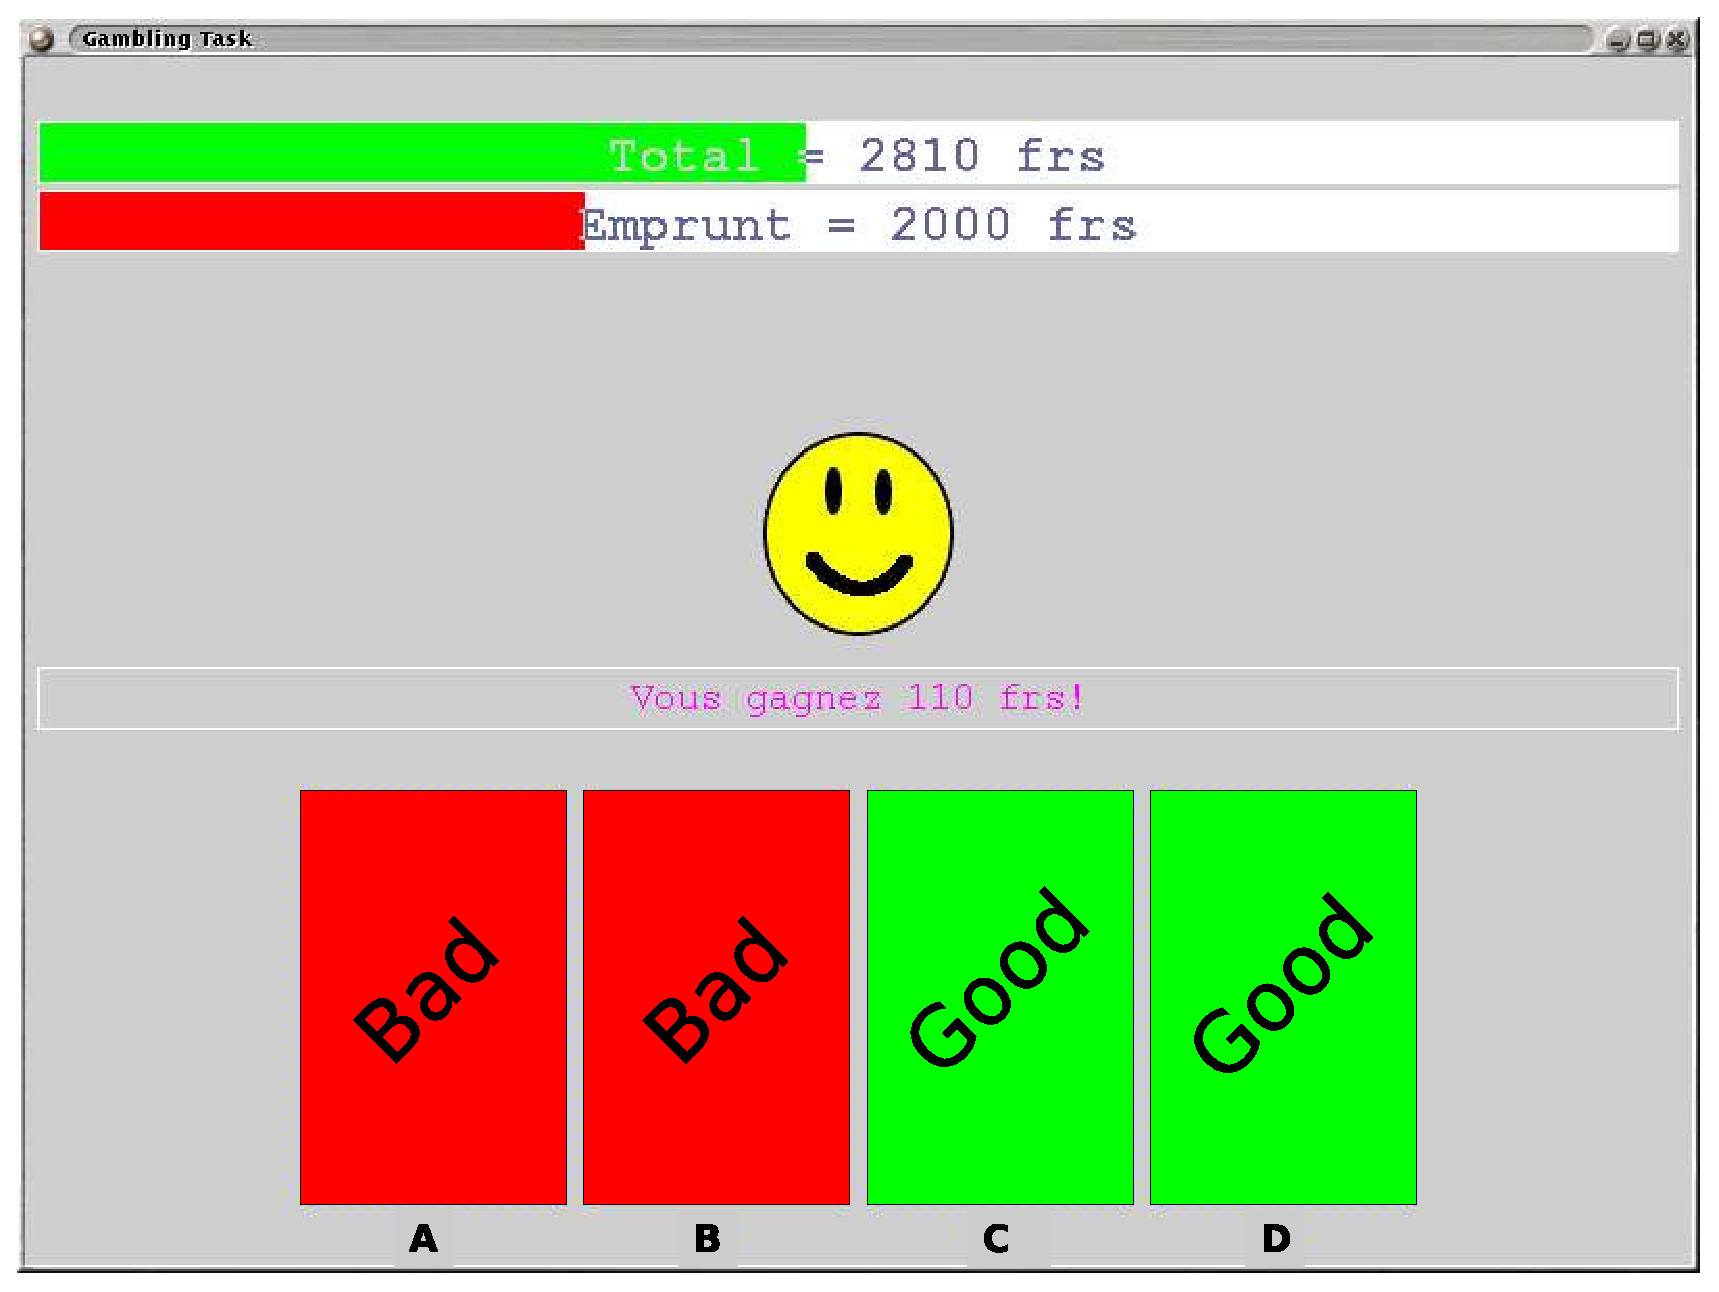
\includegraphics{Figure/GamblingTask-v1.eps}} \\
\small Version ABCD.
\end{center}
\end{textblock*}

\begin{textblock*}{110mm}(150mm,425mm)
\begin{center}
\resizebox{100mm}{!}{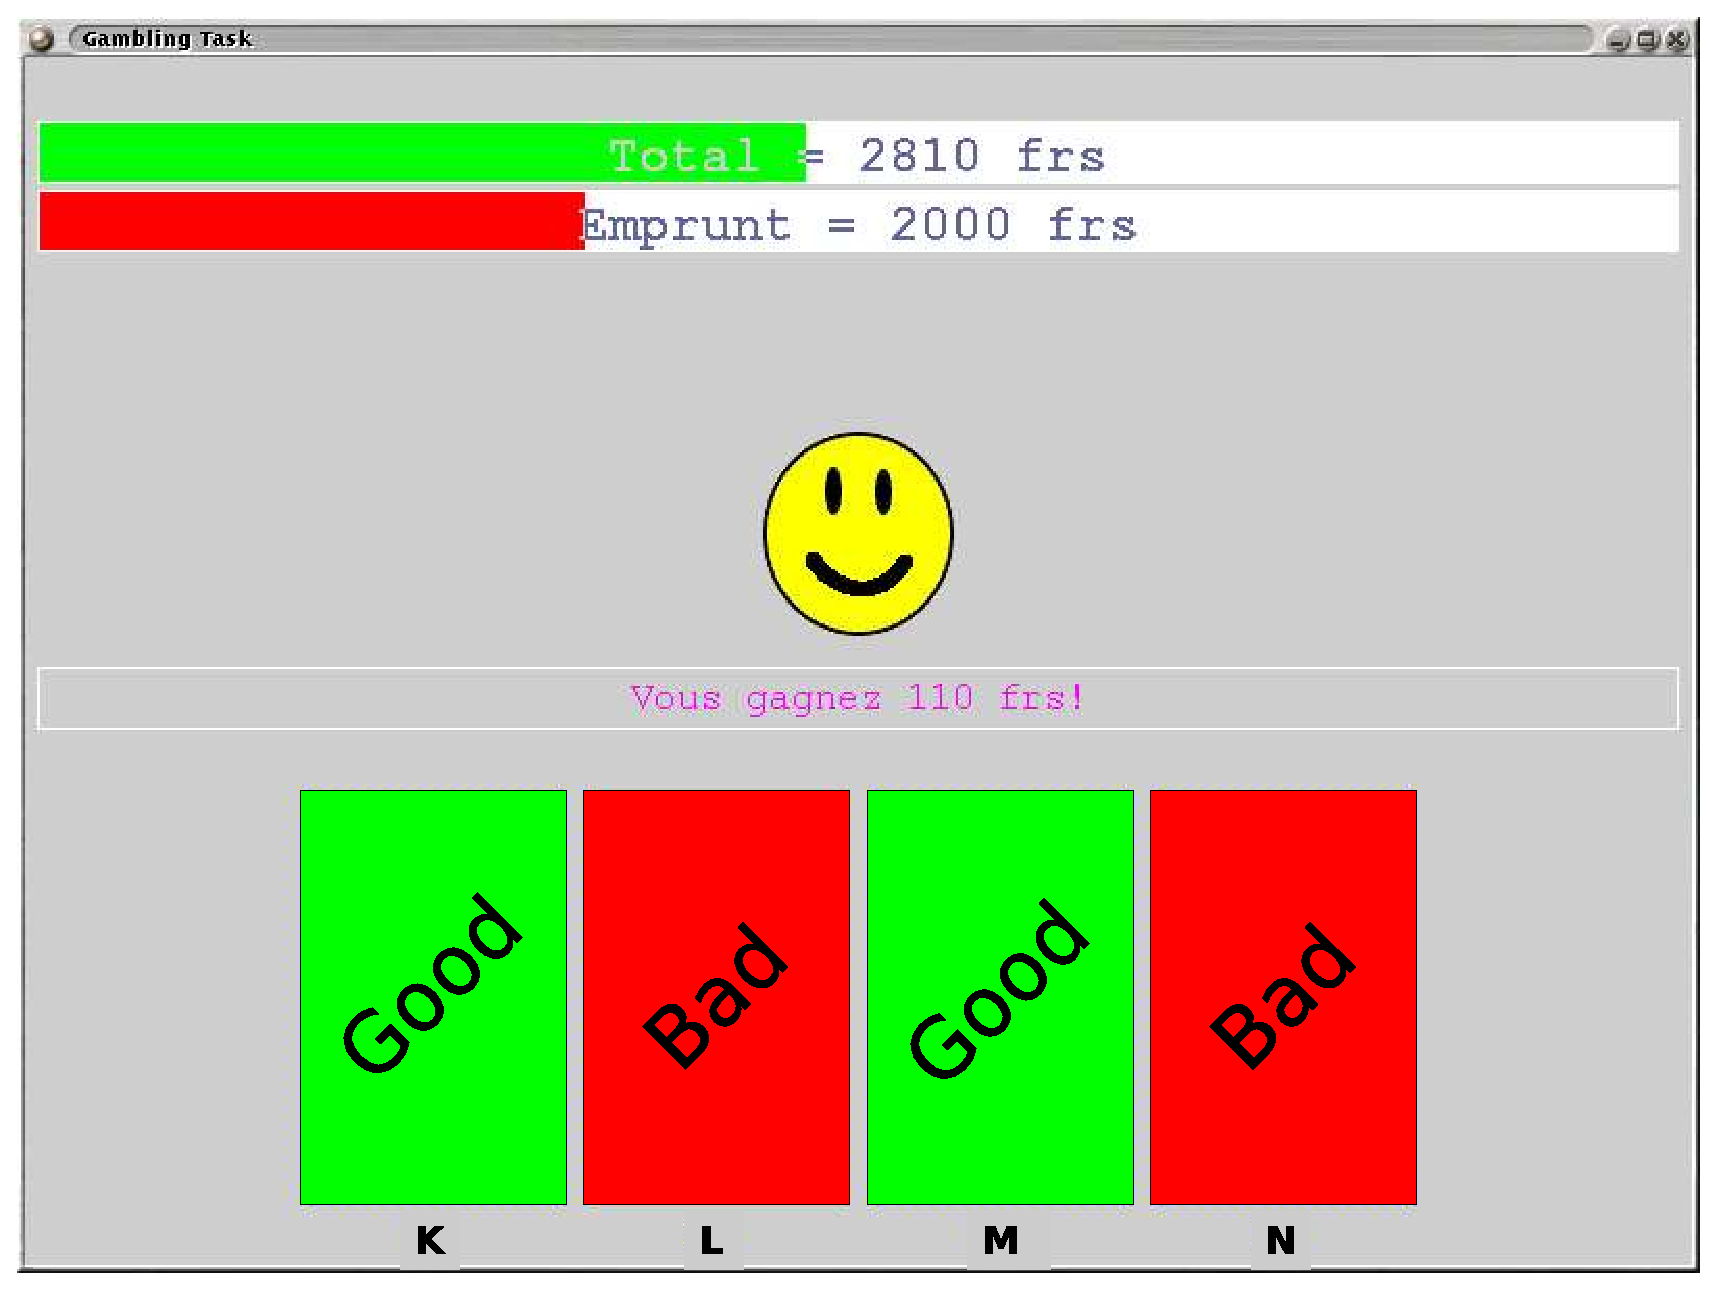
\includegraphics{Figure/GamblingTask-v2.eps}} \\
\small Version KLMN.
\end{center}
\end{textblock*}

\begin{textblock*}{110mm}(260mm,425mm)
\begin{center}
\resizebox{100mm}{!}{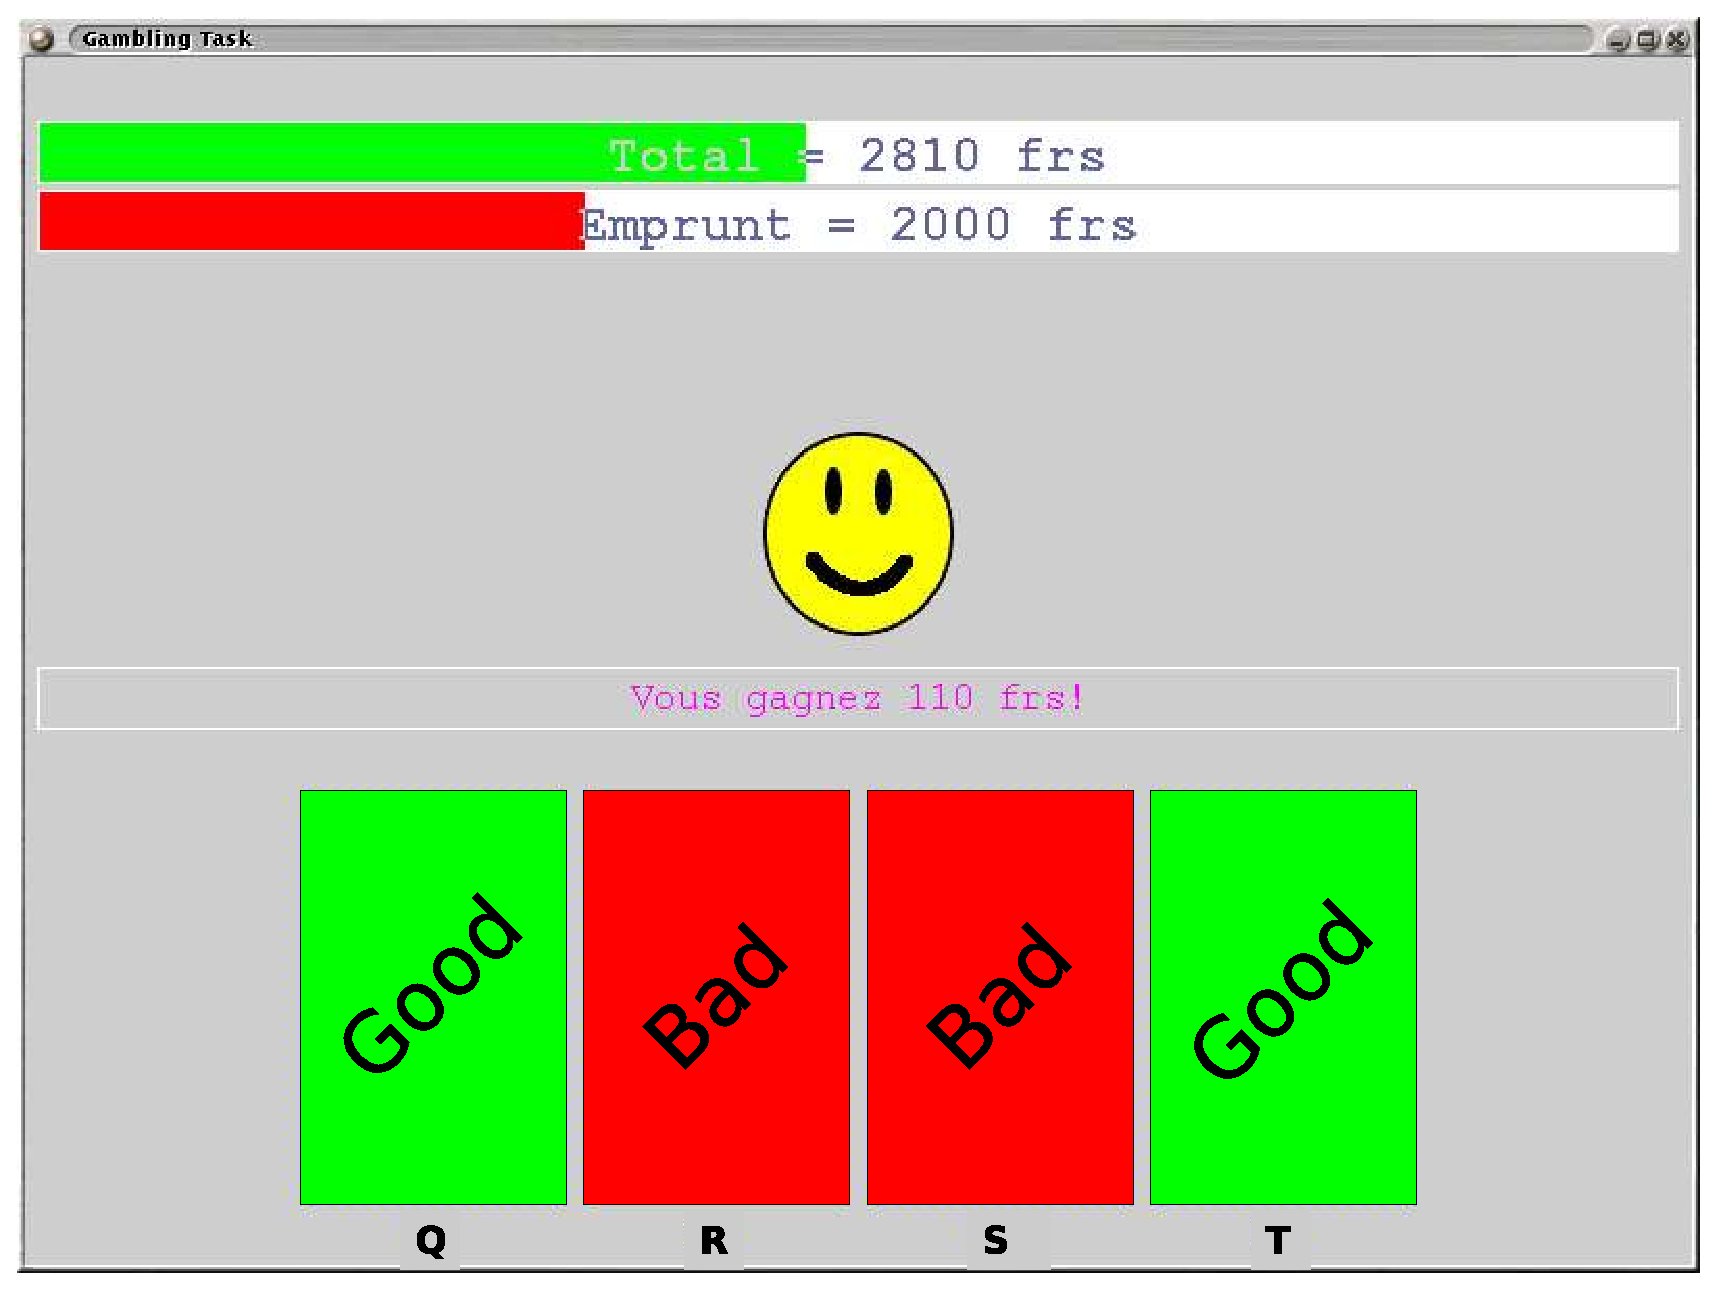
\includegraphics{Figure/GamblingTask-v3.eps}} \\
\small Version QRST.
\end{center}
\end{textblock*}

\begin{textblock*}{110mm}(40mm,520mm)
\begin{center}
\resizebox{100mm}{!}{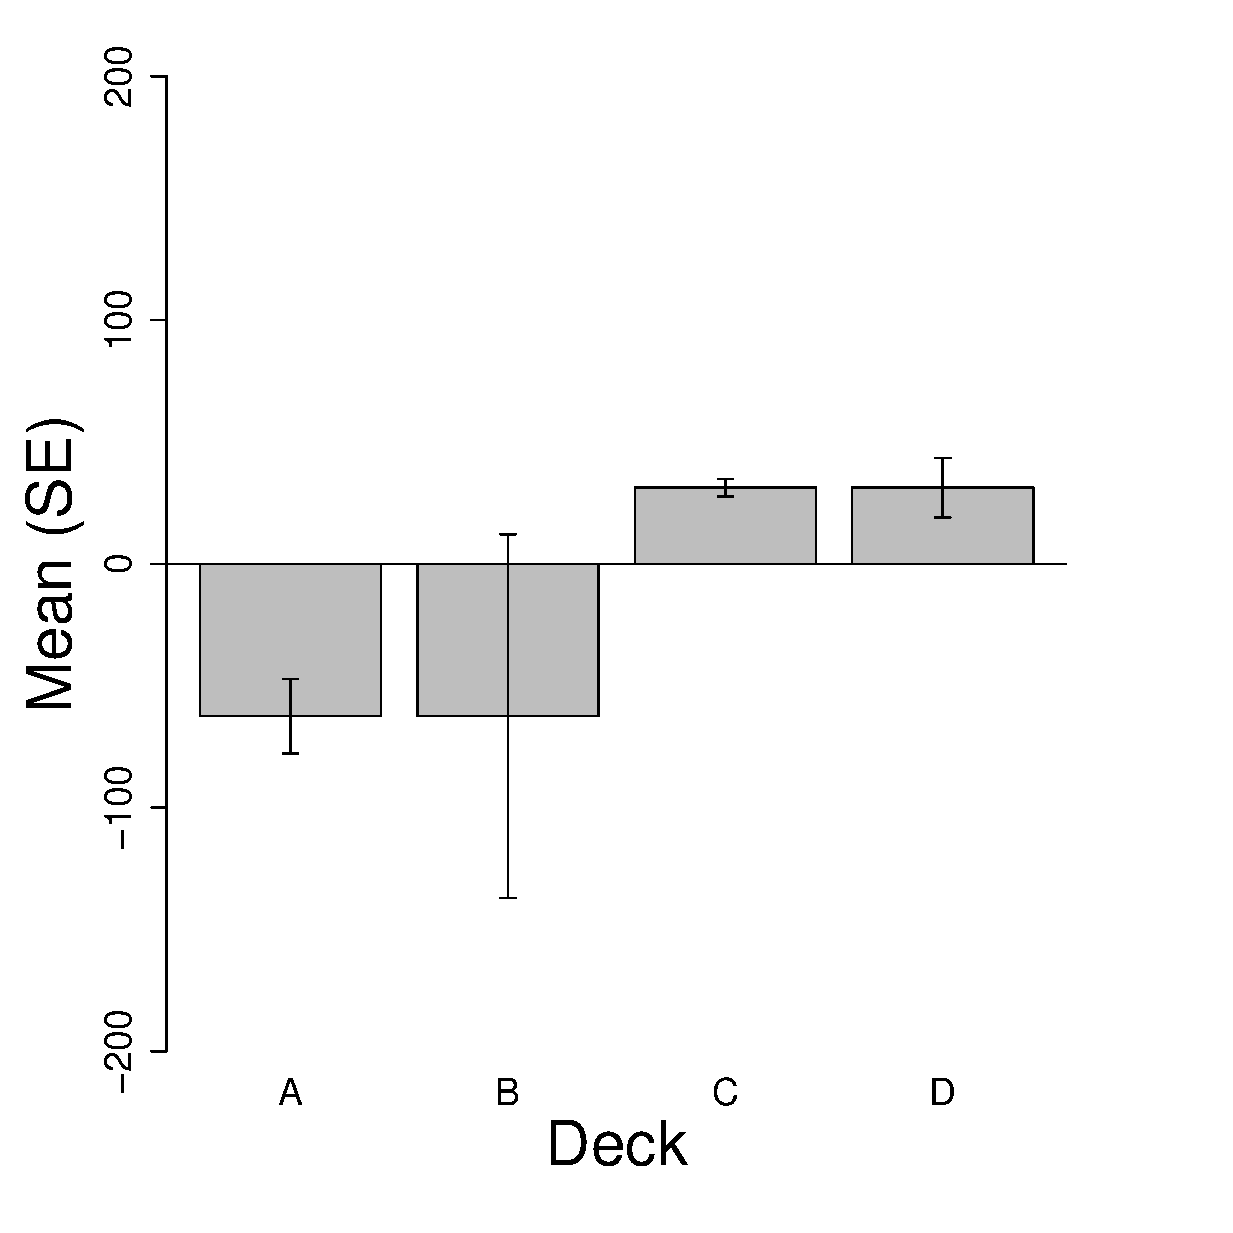
\includegraphics{Figure/MeanABCD.eps}} \\
%\small Expected gain.
\end{center}
\end{textblock*}

\begin{textblock*}{110mm}(150mm,520mm)
\begin{center}
\resizebox{100mm}{!}{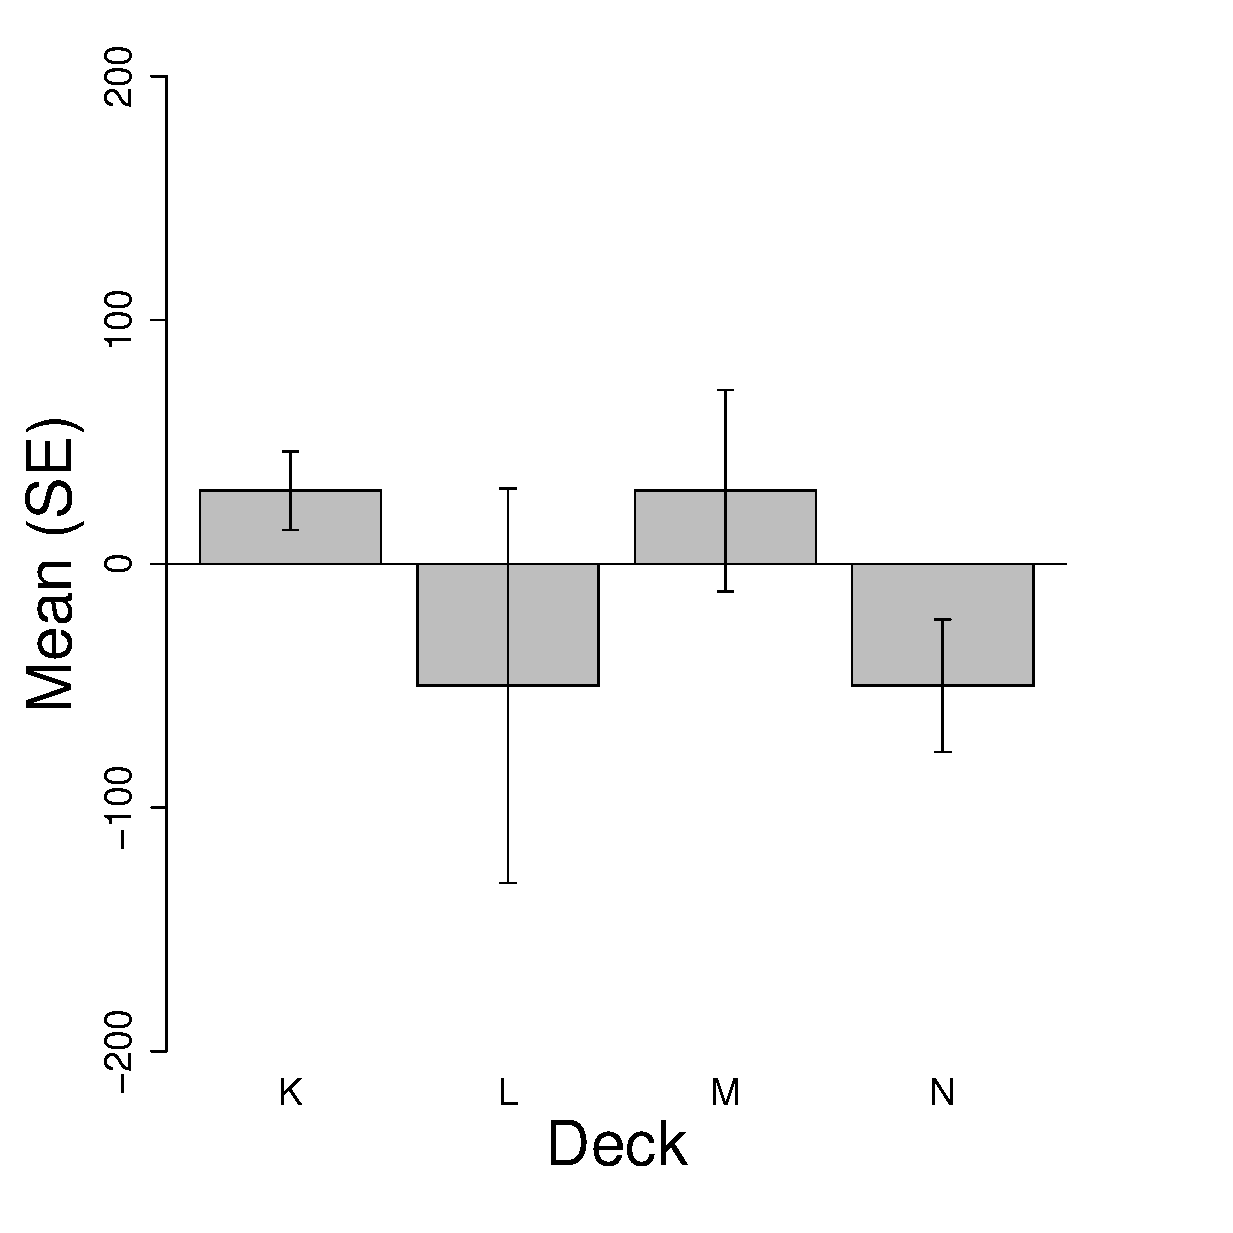
\includegraphics{Figure/MeanKLMN.eps}} \\
\small Expected gain.
\end{center}
\end{textblock*}

\begin{textblock*}{110mm}(260mm,520mm)
\begin{center}
\resizebox{100mm}{!}{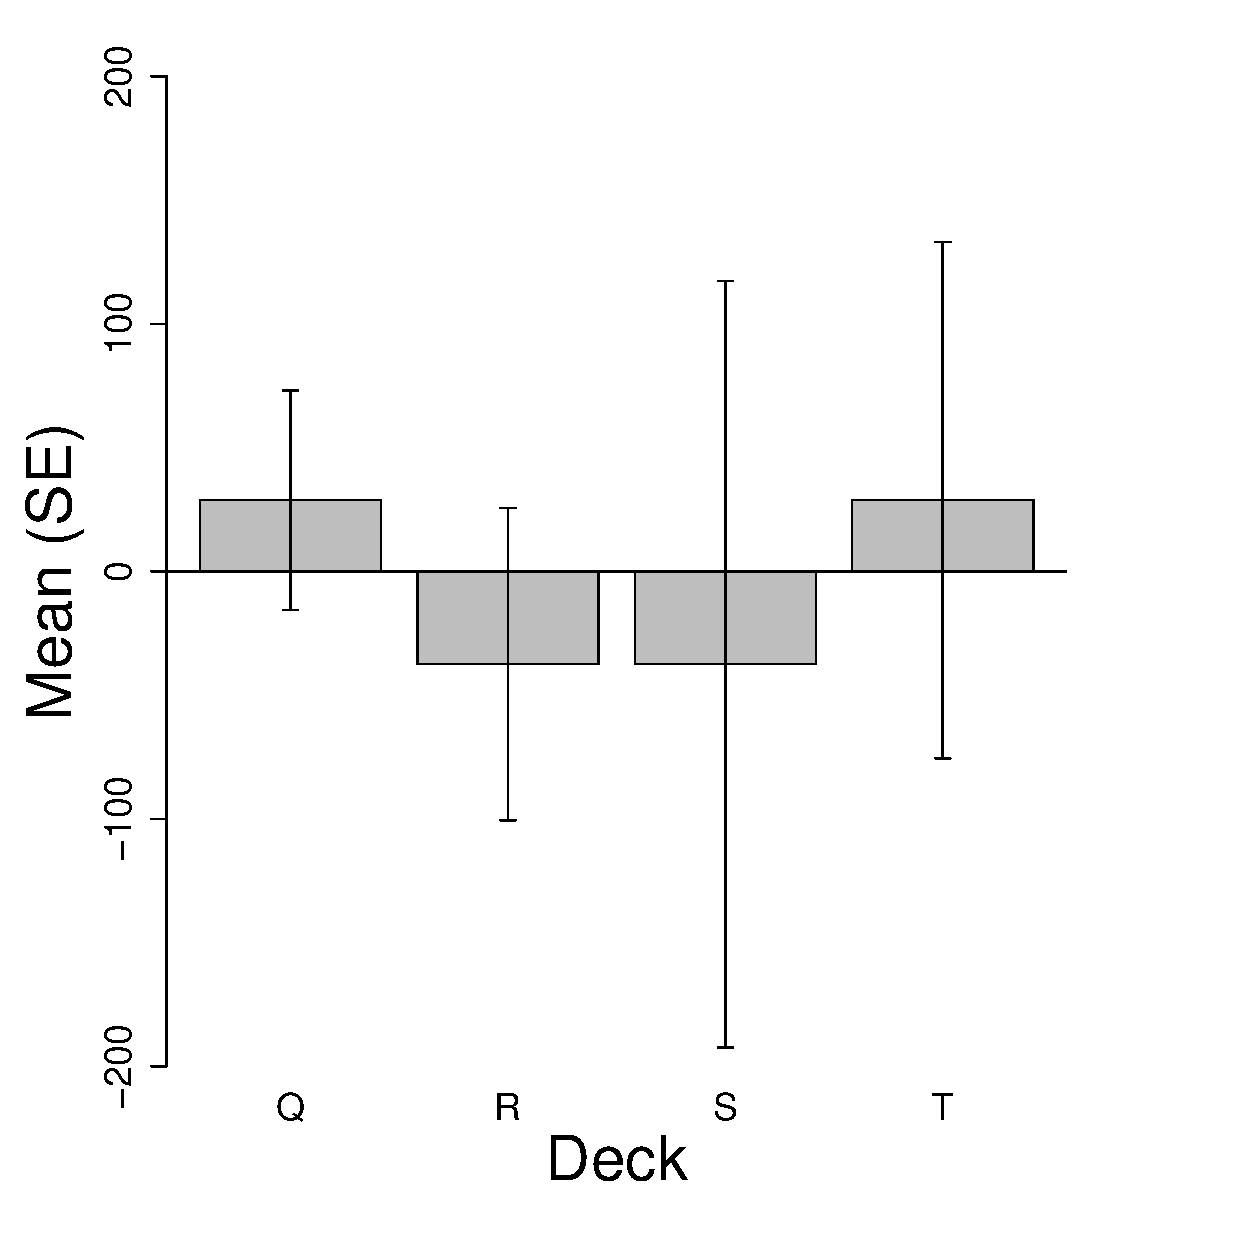
\includegraphics{Figure/MeanQRST.eps}} \\
%\small Expected gain.
\end{center}
\end{textblock*}

% Modeling decision-making
\begin{textblock*}{340mm}(40mm, 660mm)
\LHead{\bf Modeling decision-making}\medskip

\begin{itemize}
	\item Decision-making in the IGT depends on several psychological processes;
	\item Authors \shortcite{Busemeyer02} have used a reinforcement learning model with 3 parameters to explain performance in the IGT:
	\begin{enumerate}
	\item An updating rate ($0 < \tcr{\beta} < 1$);
	\item A sensitivity to reward ($0 < \tcr{\sigma} < 1$);
	\item An exploration tendency ($0 < \tcr{\tau}$).
	\end{enumerate} 
\end{itemize}
\end{textblock*}

% Aims
\begin{textblock*}{340mm}(40mm, 780mm)
\LHead{\bf Rational and aims}\medskip

\begin{itemize}
	\item The ABCD version has been used to model decision-making; 
	\item This is problematic because it has been shown that model parameters are unreliable when estimated on only 100 trials \shortcite{Dacremont06}; 
	\item Based on this limitation, our aims were twofolds:
	\begin{enumerate}
	\item See if the model parameters are more reliable when estimated on the 3 versions of the IGT offering 300 trials (simulation);
	\item Estimate the model parameters on data collected with the 3 versions of the IGT and explore their relationships with impulsivity (application on real data). 
	\end{enumerate} 
\end{itemize}

\end{textblock*}

% Simulated decisions
\begin{textblock*}{340mm}(40mm,920mm)
\LHead{\bf Simulated decisions}\medskip

{\bfseries Reinforcement learning algorithm:}\smallskip 
\begin{algorithmic}[1]
   \STATE Initialize action probability $p_i = 0.25$, \, $i=1,\ldots,4$
   \STATE Initialize action value $\mathtt{ActVal}_i = 0$, \, $i=1,\ldots,4$
   \FOR {$k = 1:\tcr{n}$}
      \STATE Select deck $i$ according to $p$
      \STATE $\mathtt{RewVal} = (\tcr{\sigma}\,\mathtt{Reward}_i + (1-\tcr{\sigma})\,\mathtt{Punish}_i)$
      \STATE $\mathtt{PredErr} = \mathtt{RewVal} - \mathtt{ActVal}_i$
      \STATE $\mathtt{ActVal}_i = \mathtt{ActVal}_i + \tcr{\beta} \, \mathtt{PredErr}$
      \STATE $x_i = \exp(\mathtt{ActVal}_i \, / \tcr{\tau})$, \, $i=1,\ldots,4$
      \STATE Update action probability $p_i = x_i / \sum_{j=1}^4 x_j$
   \ENDFOR
\end{algorithmic}
\end{textblock*}

% Second column

\begin{textblock*}{340mm}(420mm,220mm)
{\bfseries Simulation on version ABCD, KLMN, and QRST:}
\begin{itemize}
\item Parameters in the learning algorithm are fixed to: a moderate updating rate ($\tcr{\beta} = .10$), a low sensitivity to reward ($\tcr{\sigma} = .40$), and a tendency to explore the environment ($\tcr{\tau}~=~50$);
\item The learning algorithm is used to simulate the decision of one ``subject'';
\item Results indicate that the probability to select the good decks increases with trials in the ABCD and KLMN version $\Rightarrow$ the algorithm learns to take advantageous decisions;
\item There is no learning in the QRST version $\Rightarrow$ this result reflects the difficulty of version QRST.
\end{itemize}
\begin{center}
\resizebox{320mm}{!}{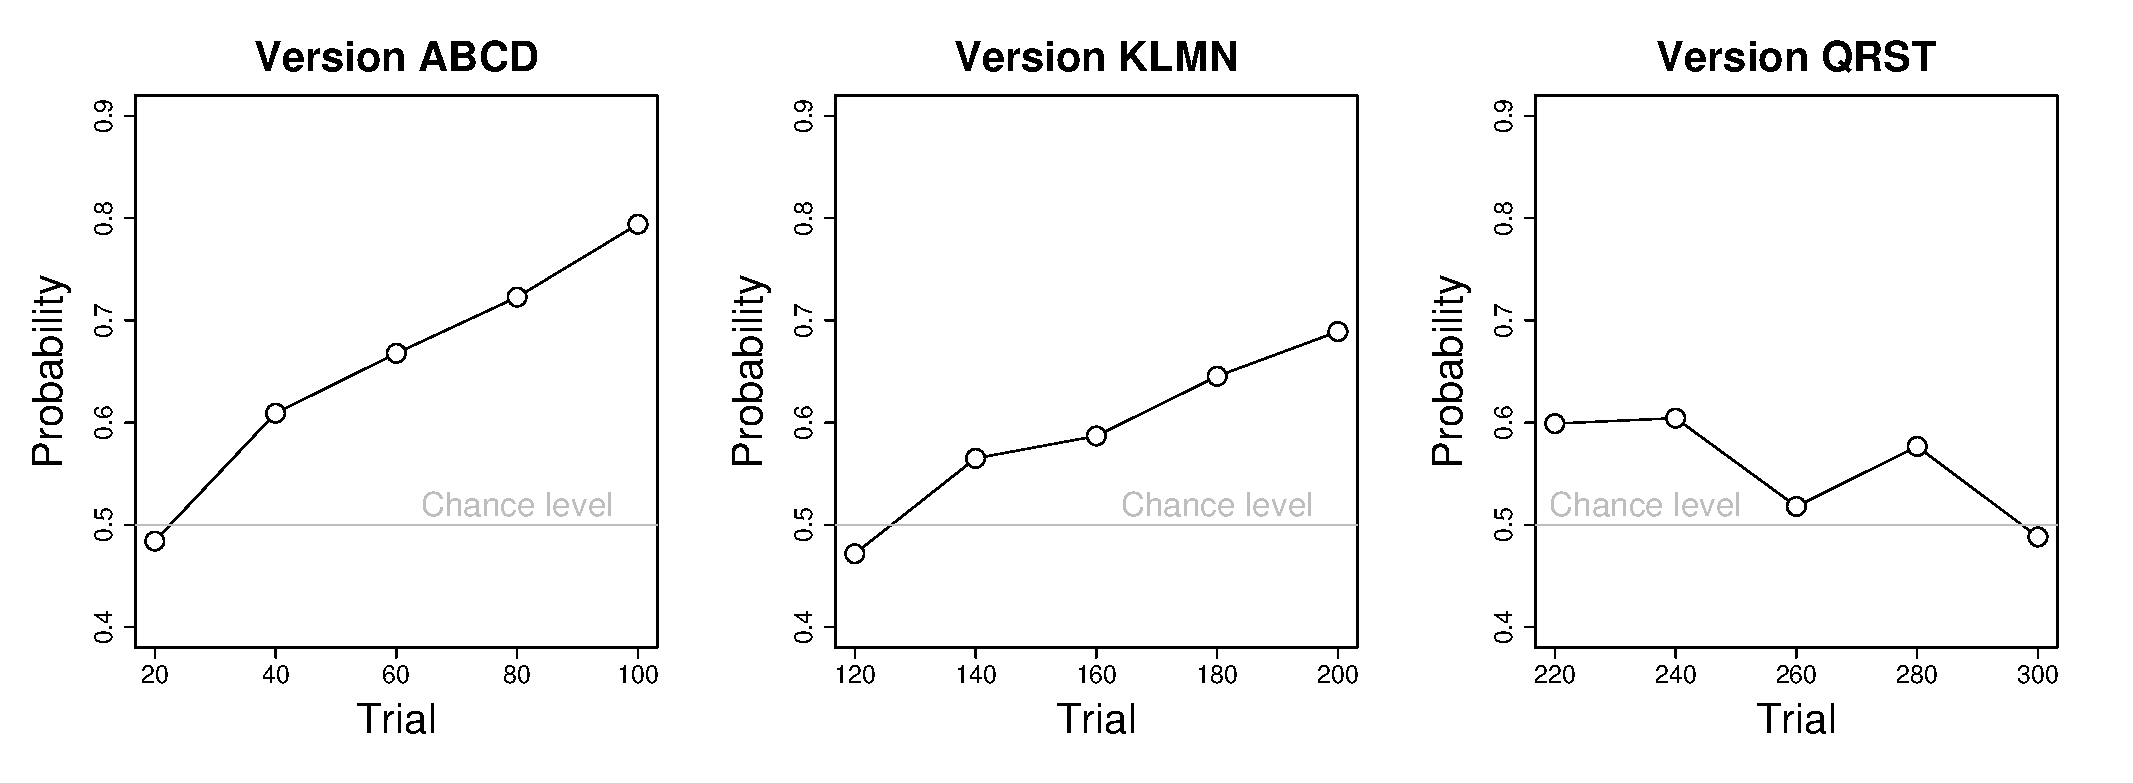
\includegraphics{Figure/ProbPointAkq10_60_50_100.eps}} \\
\small Probability to select the good decks.
\end{center}
\end{textblock*}


% Repeat estimation + Figure 3
\begin{textblock*}{340mm}(420mm,460mm)
{\bfseries Estimation on version ABCD:}
\begin{itemize}
\item Parameters in the learning algorithm are fixed to the same values: ($\tcr{\beta}=.10$, $\tcr{\sigma}=.40$, $\tcr{\tau}=50$);
\item Decisions for 100 ``subjects'' are simulated with the learning algorithm on version ABCD;
\item For each ``subject'', the models parameters are estimated by mean of maximum likelihood;
\item Results show a high variability of the estimated parameters around the fixed parameters.
\end{itemize}
\begin{center}
\resizebox{320mm}{!}{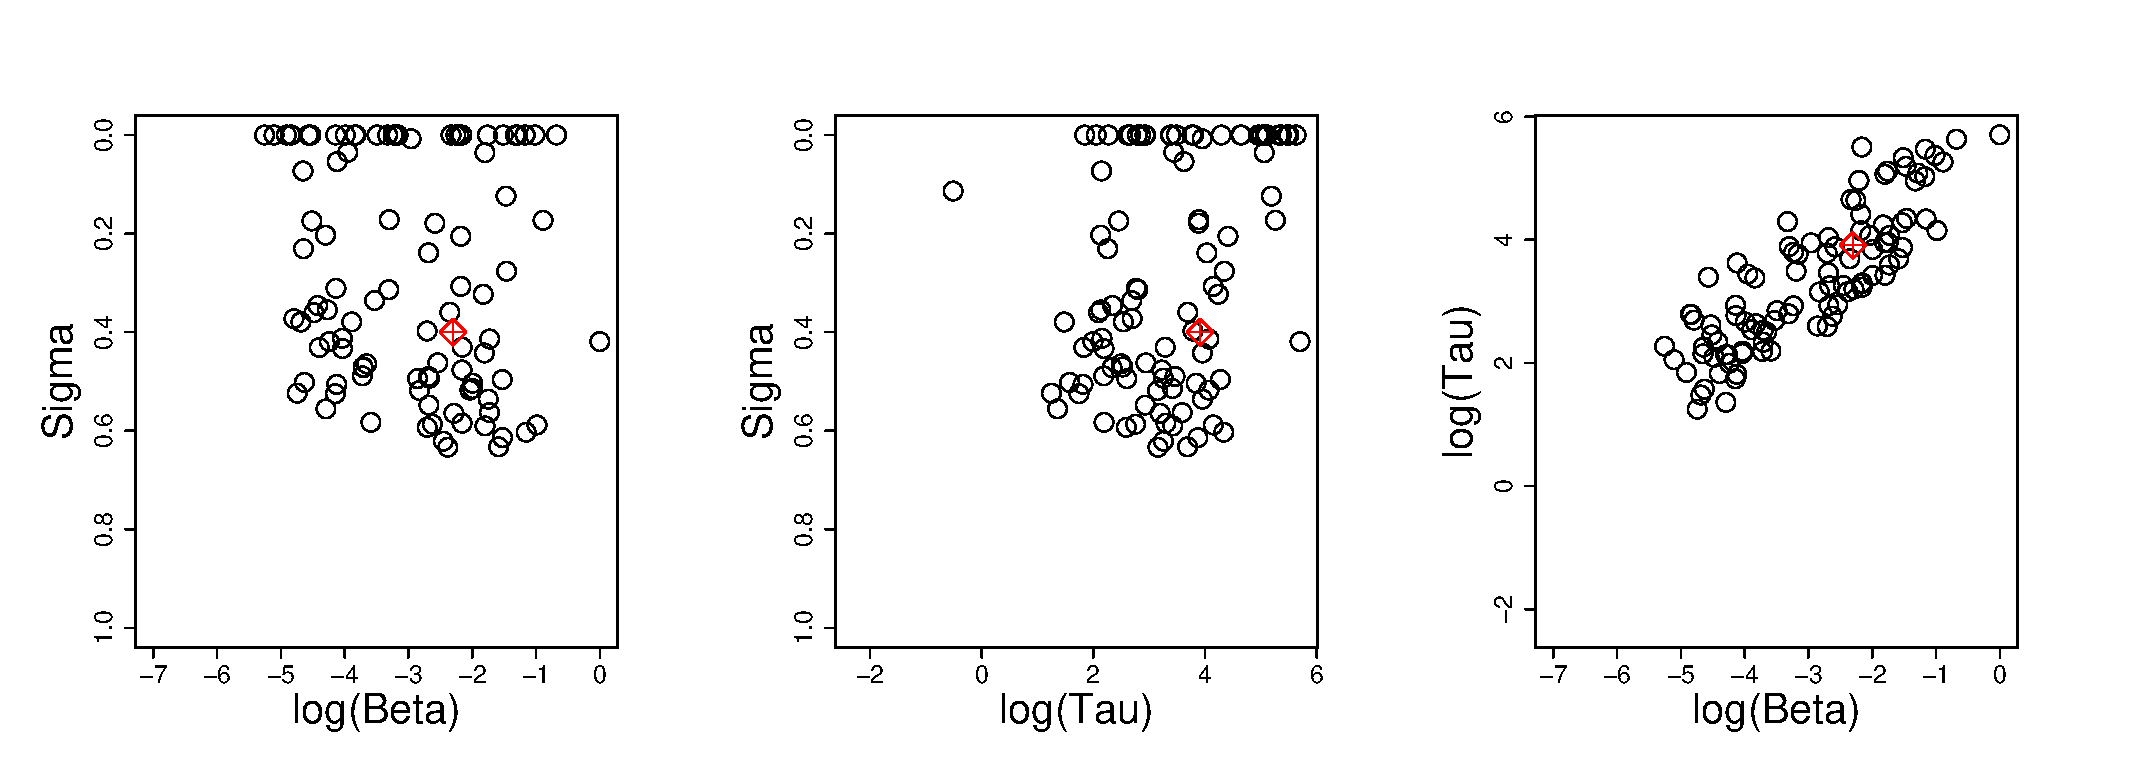
\includegraphics{Figure/SpreadA10_60_50_100.eps}} \\
\small The red point = fixed parameters. Small points = estimated parameters for 100 ``subjects''.
\end{center} \medskip
\end{textblock*}


% Repeat estimation + Figure 3
\begin{textblock*}{340mm}(420mm,680mm)
{\bfseries Estimation on version ABCD, KLMN, and QRST:}
\begin{itemize}
\item The same strategy is used, but decisions for the 100 ``subjects'' are simulated on the 3 versions;
\item Results show a reduced variability of the estimated parameters around the fixed parameters $\Rightarrow$ the reliability of the estimated parameters increased with the use of the 3 versions;
\end{itemize}
\begin{center}
\resizebox{320mm}{!}{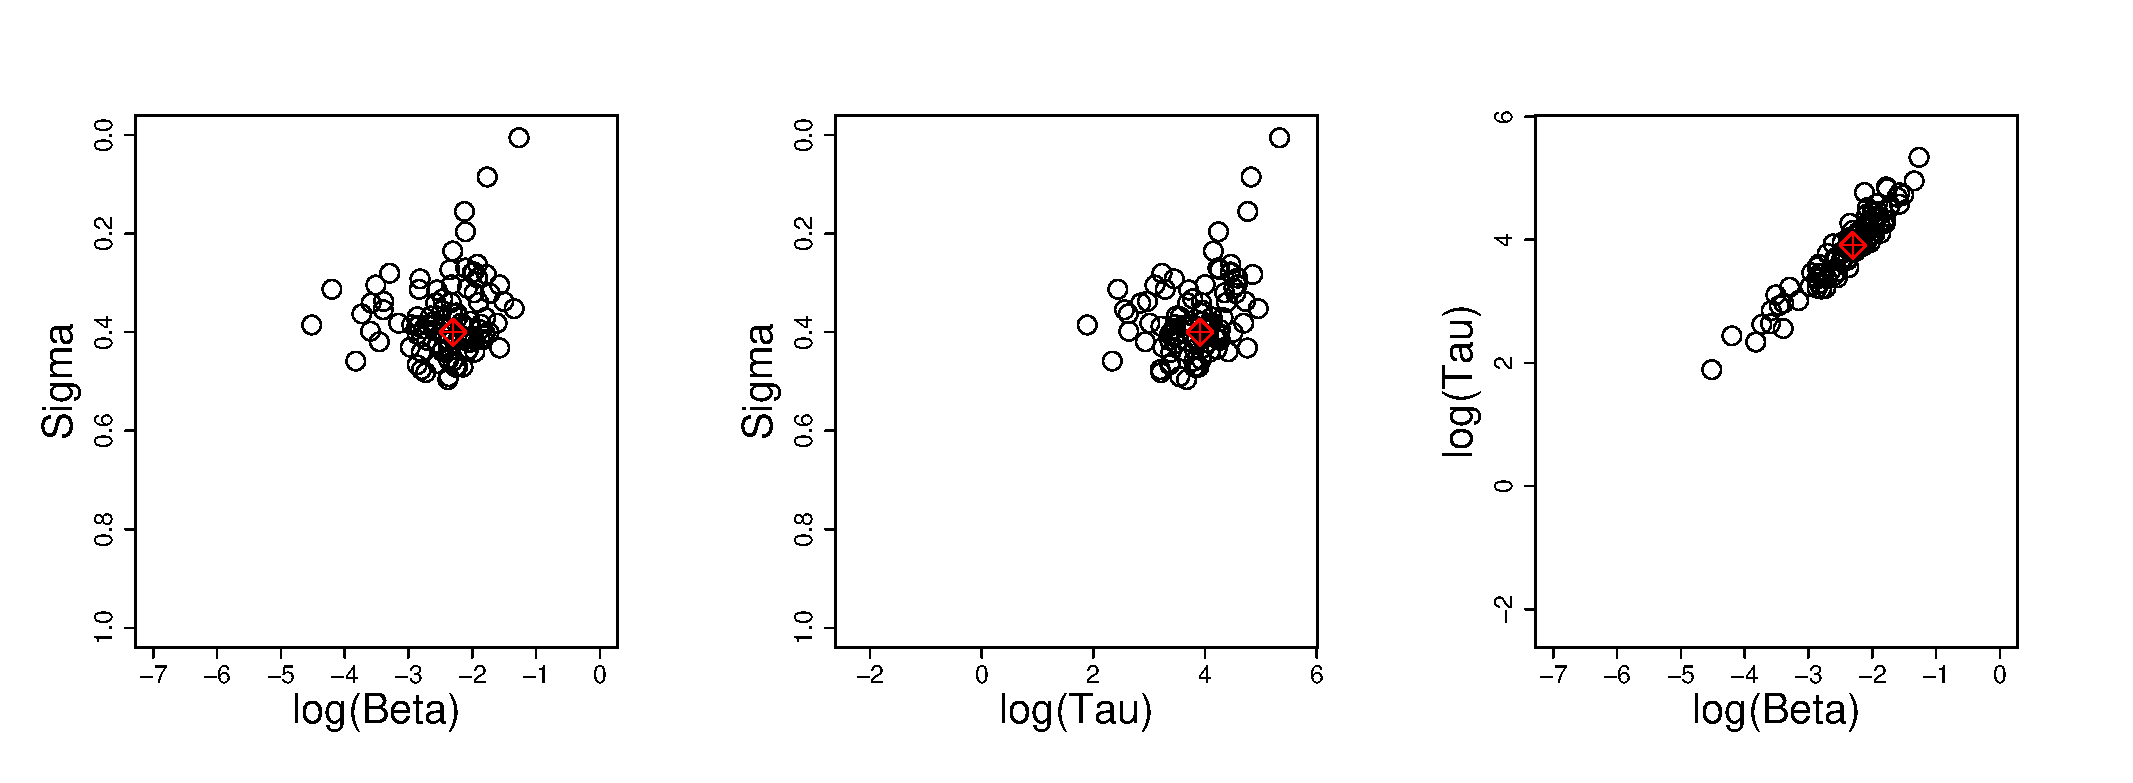
\includegraphics{Figure/SpreadAkq10_60_50_100.eps}} \\
\small The red point = fixed parameters. Small points = estimated parameters for 100 ``subjects''.
\end{center} \medskip
\end{textblock*}

% Estimation from real data + Figure 4
\begin{textblock*}{340mm}(420mm,885mm)
\LHead{\bf Parameter estimation from real data}\medskip
\begin{itemize}
\item 61 adults completed successively the 3 versions of IGT and the UPPS Impulsive Behavior Scale \shortcite{Whiteside01};
\item The model parameters ($\tcr{\beta}$, $\tcr{\sigma}$, $\tcr{\tau}$) were estimated for each subject on the 300 trials;
\item A significant correlation was found between lack of Premeditation (one aspect of impulsivity) and sensitivity to reward, r = .34*, 95\% CI = (.09, .55);
\item This results corroborate the hypothesis of a higher sensitivity to reward in impulsive subjects \shortcite{Corr95};
\end{itemize}
\end{textblock*}


% Conclusion
\begin{textblock*}{340mm}(420mm,1010mm)
\LHead{\bf Conclusions}\medskip

\begin{itemize} 
\item Simulation revealed that the use of 3 versions of the IGT gives a more accurate estimation of the parameters;
\item An application on real data showed a meaningfull relationship between one aspect of impulsivity and decision-making.
\end{itemize}
\end{textblock*}

% References
\begin{textblock*}{720mm}(40mm,1065mm)
\bibliographystyle{apacite}
\bibliography{Poster}
\end{textblock*}

\end{document}
